
        \documentclass[tikz]{standalone}
        \usepackage{tikz}
        \usetikzlibrary{trees,shapes.geometric,positioning}
        
        \begin{document}
        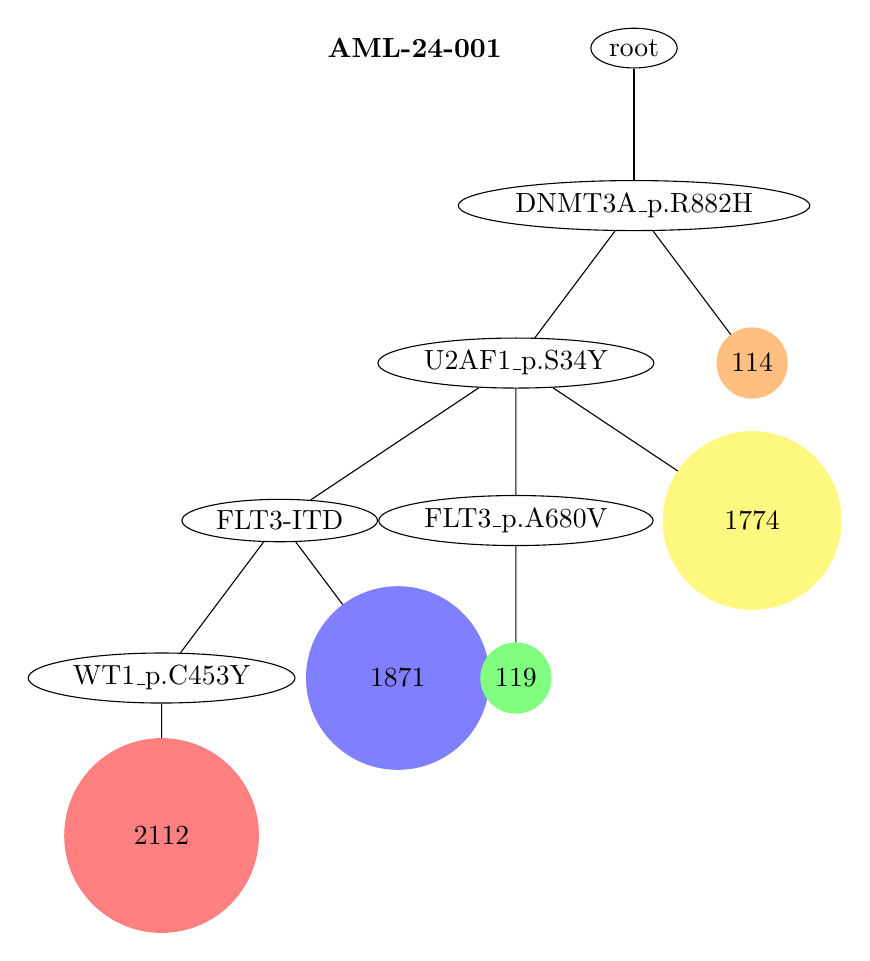
\begin{tikzpicture}[
            sizenode/.style 2 args={circle, draw=#1, fill=#1, minimum size=#2},
            treenode/.style={ellipse, draw, inner sep=2pt, align=center},
            level 1/.style={level distance=2cm,sibling distance=3cm},
            level 2/.style={level distance=2cm,sibling distance=3cm}
        ]
        
        \node [treenode] (root) {root}
	child {node [treenode] {DNMT3A\_p.R882H}
		child {node [treenode] {U2AF1\_p.S34Y}
			child {node [treenode] {FLT3-ITD}
				child {node [treenode] {WT1\_p.C453Y}
					child {node [sizenode={red!50}{2.4594316186372973cm}] {2112}}
				}
				child {node [sizenode={blue!50}{2.3180291940324875cm}] {1871}}
			}
			child {node [treenode] {FLT3\_p.A680V}
				child {node [sizenode={green!50}{0.3260208495212452cm}] {119}}
			}
			child {node [sizenode={yellow!50}{2.256959170860382cm}] {1774}}
		}
		child {node [sizenode={orange!50}{0.3137075880823939cm}] {114}}
	};

\node [left=1cm of root] {\textbf{AML-24-001}};


        \end{tikzpicture}
        \end{document}
        